\documentclass[hidelinks, 12pt, a4paper]{article}

\usepackage[utf8]{inputenc}
\usepackage[margin=1.5cm]{geometry}
\usepackage{graphicx}
\usepackage{setspace}
\usepackage[T1]{fontenc}
\usepackage{tocloft}
\usepackage{todonotes}
\usepackage{epstopdf} 
\usepackage{hyperref}
\usepackage{float}
\usepackage{titlesec}
\usepackage{listings}
\usepackage{multirow}
\usepackage{xcolor}
\usepackage{mwe}
\usepackage{hyperref}
\onehalfspacing
\usepackage[english]{babel}
\usepackage{fancyhdr}
\usepackage{enumitem}

\pagestyle{fancy}
\fancyhf{}
\rhead{blulancetech@gmail.com}
\lhead{Carpool}
\rfoot{Page \thepage}

\author{}
\date{}
\title
{
	
\includegraphics[width=6cm]{images/up_logo.jpg} \\
	Department of Computer Science \\
	Faculty of Engineering, Built Environment \& IT\\
	University of Pretoria \\
	\vspace{0.5cm}
	\Huge COS301 -
	Software Engineering\\
	\vspace{1cm}
	{\Huge Carpool}\\
	\begin{Large}
	User Manual
	\end{Large}
	\vspace{0.5cm}
	
    \begin{center}
    \noindent
    
\includegraphics[width=6cm]{images/company_logo.png} 
    \vspace{0.5cm}
    \begin{table}[h]
    \centering
    \begin{tabular}{|l|l|l|}
    \hline
    Name  & Student Number\\ \hline
    Benjamin Osmers & u16068344 \\ \hline
    Ashleigh Govender &  U20528834      \\ \hline
    Joshua Brink  & U19185678 \\ \hline
    Jason Antalis     & U19141859     \\ \hline
    Wesley Pachai & U20578688    \\ \hline
            
    \end{tabular}
    \end{table}
    \end{center}
    }

\begin{document}
\maketitle


\newpage
\tableofcontents
\newpage

\section{Introduction}
This document serves as an instruction manual for a user to run the Carpool Application. The document specifies what the user needs in order to run the application as well as how the user can navigate through the application.

\section{Requirements}
A smart mobile device (Android or ios) that has locational services as well as constant access to the internet.\\
The device should be small and easily mobile.

\section{Navigation}
\subsection{Authentication}
\subsubsection{Landing Page}
\begin{center}
  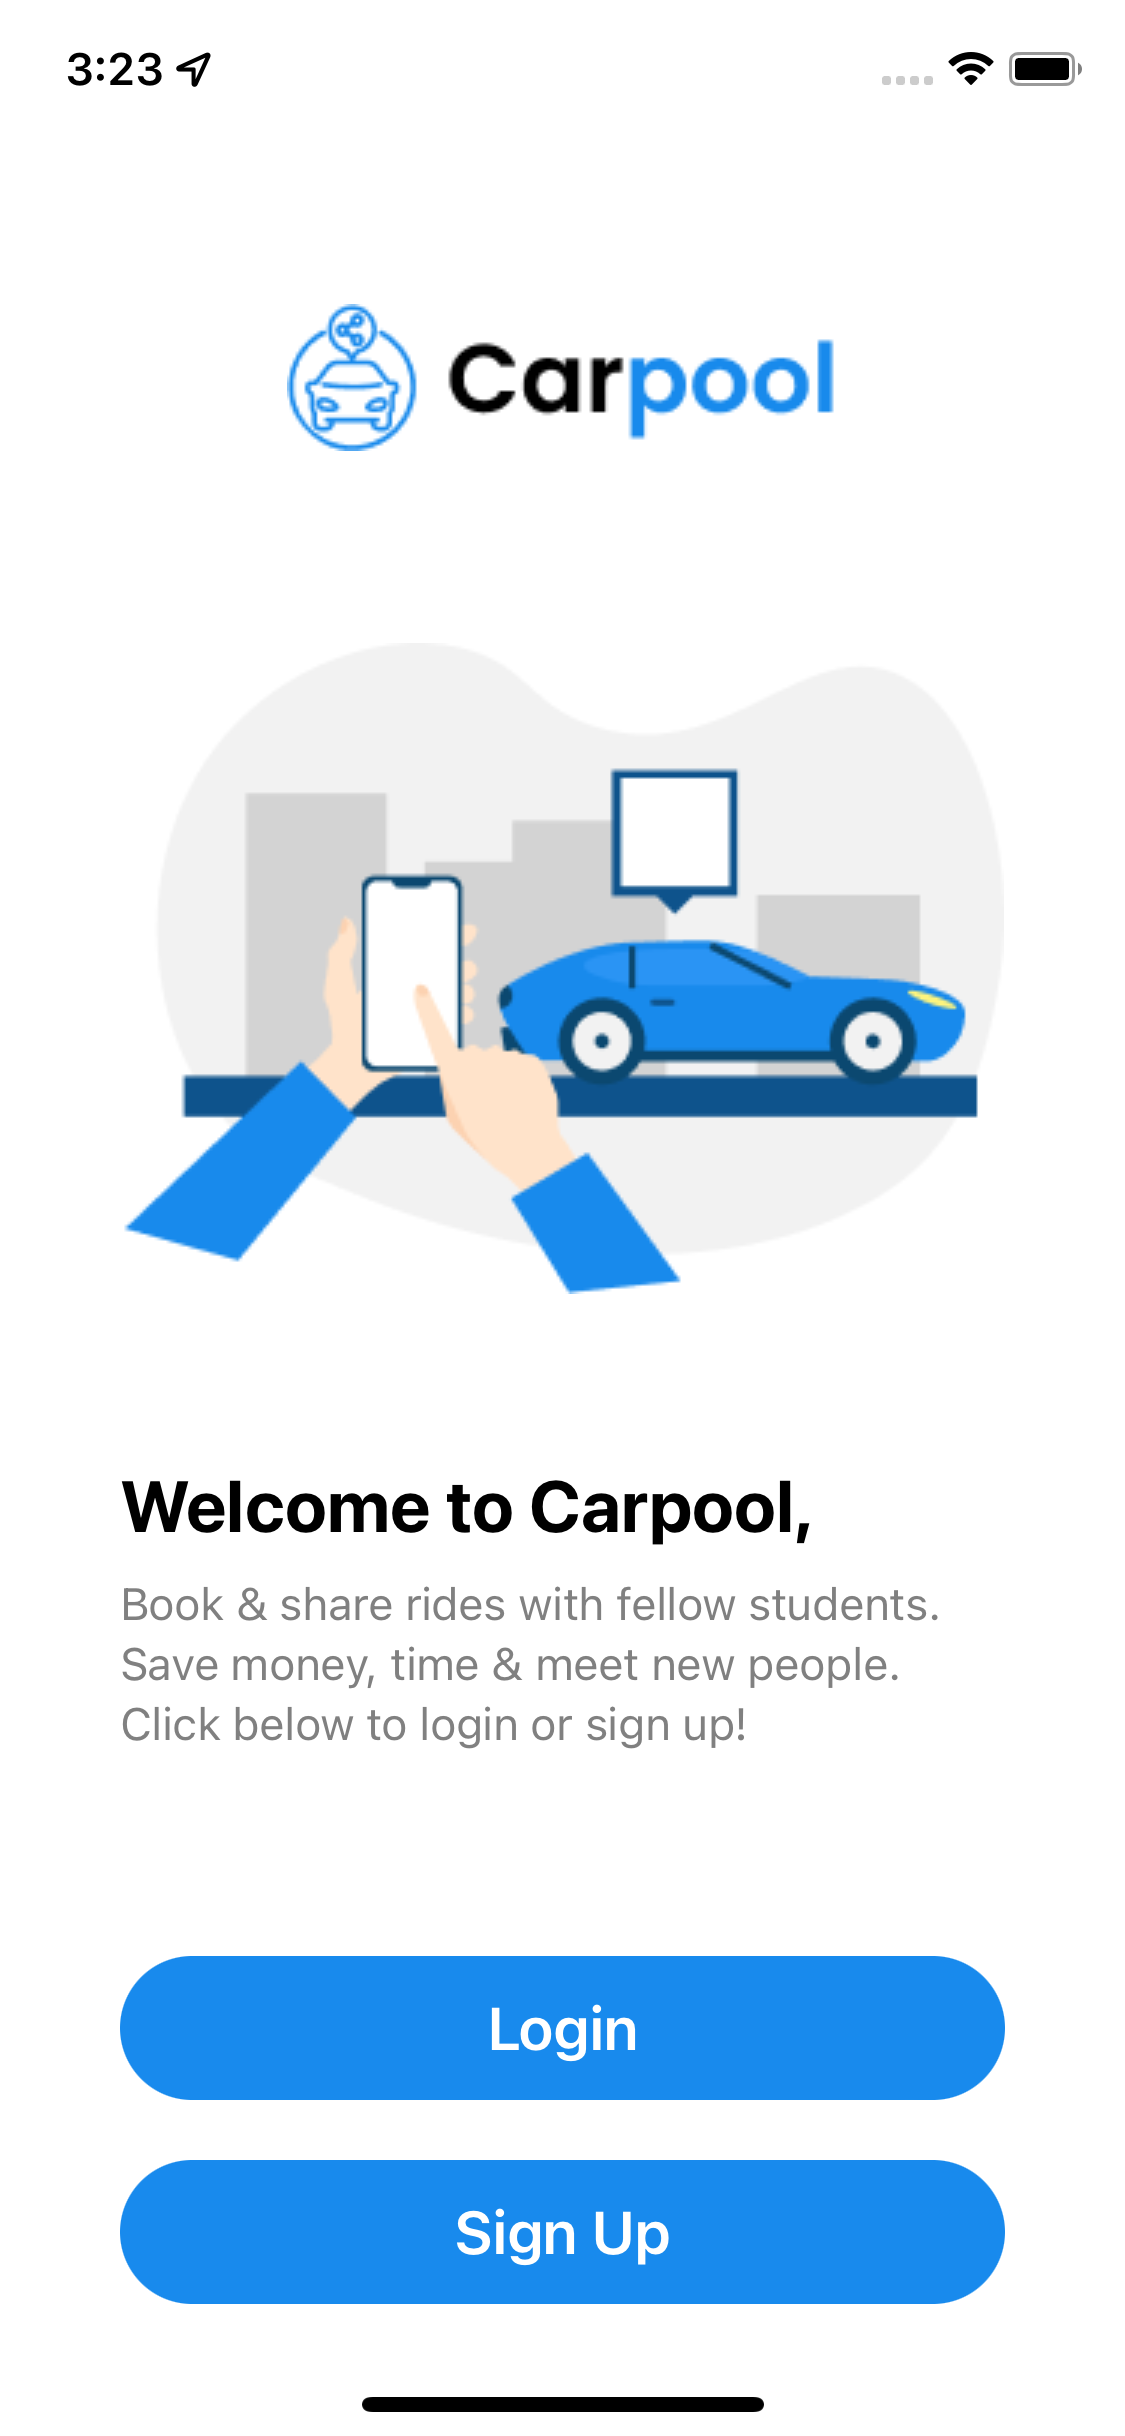
\includegraphics[height=10cm]{images/Simulator Screen Shot - iPhone X - 2022-06-10 at 03.23.06.png}
\end{center}
\subsubsection{Login Page}
\begin{center}
  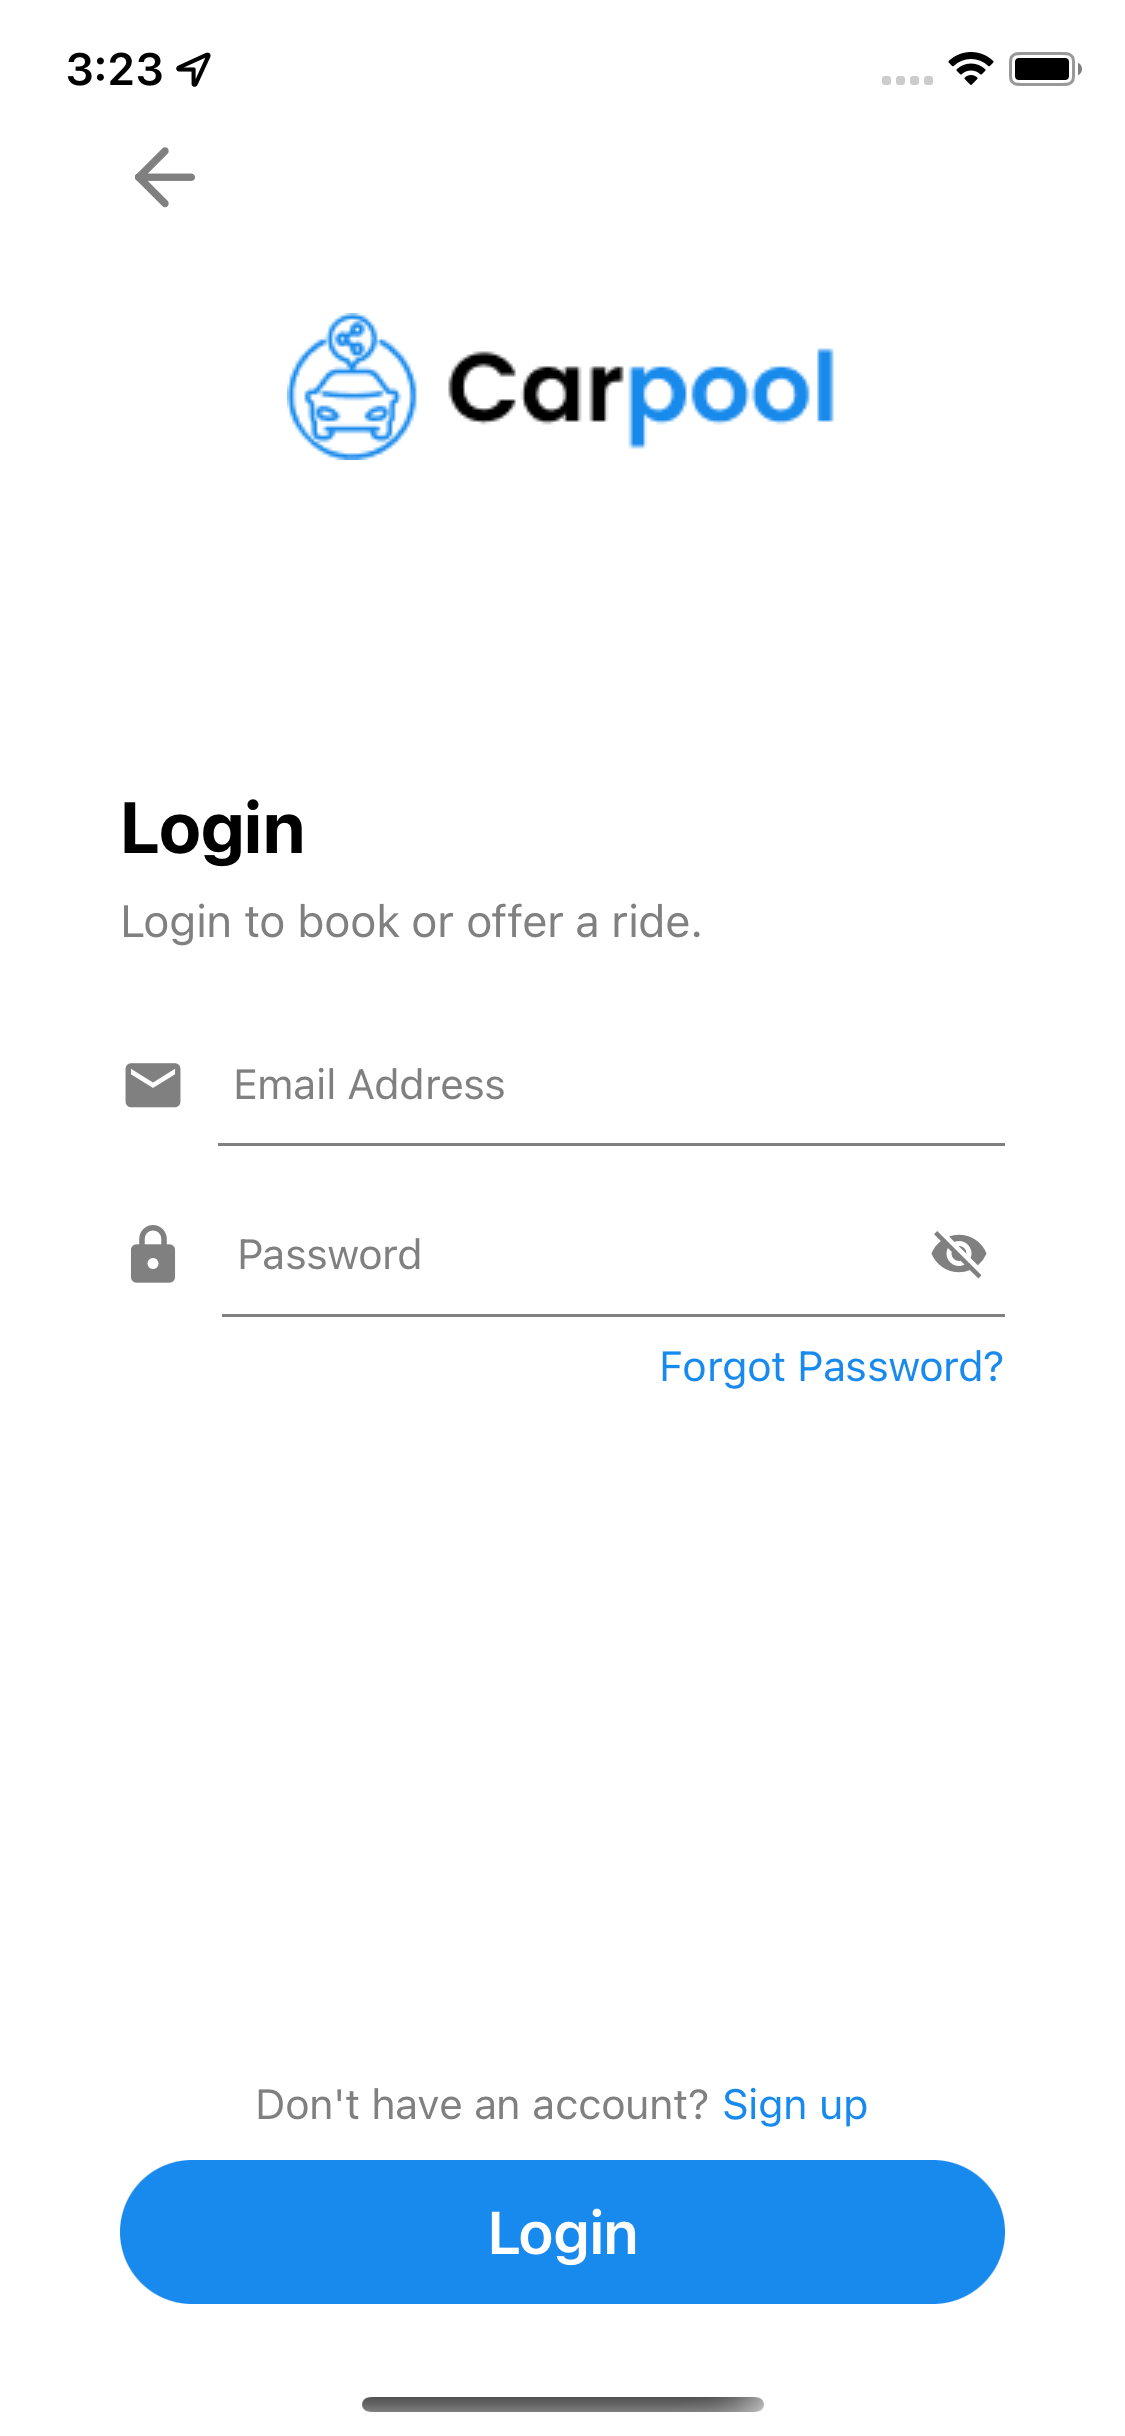
\includegraphics[height=10cm]{images/Simulator Screen Shot - iPhone X - 2022-06-10 at 03.23.09.png}
\end{center}
\vspace{1cm}
\subsubsection{Sign-up}
\begin{center}
  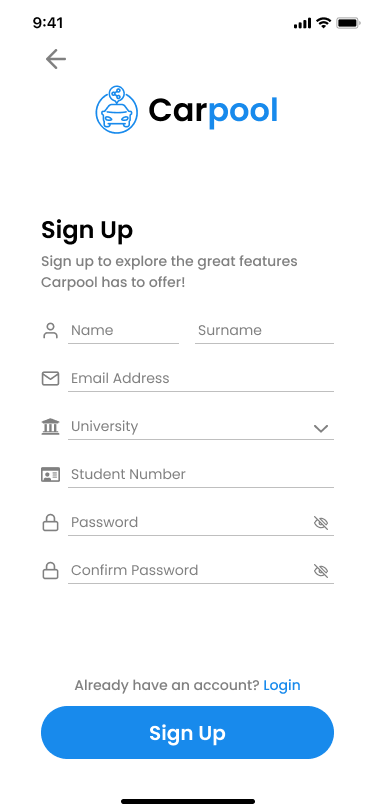
\includegraphics[height=10cm]{images/Register.png}
\end{center}
\vspace{1cm}
\subsubsection{Forgot Password}
\begin{center}
  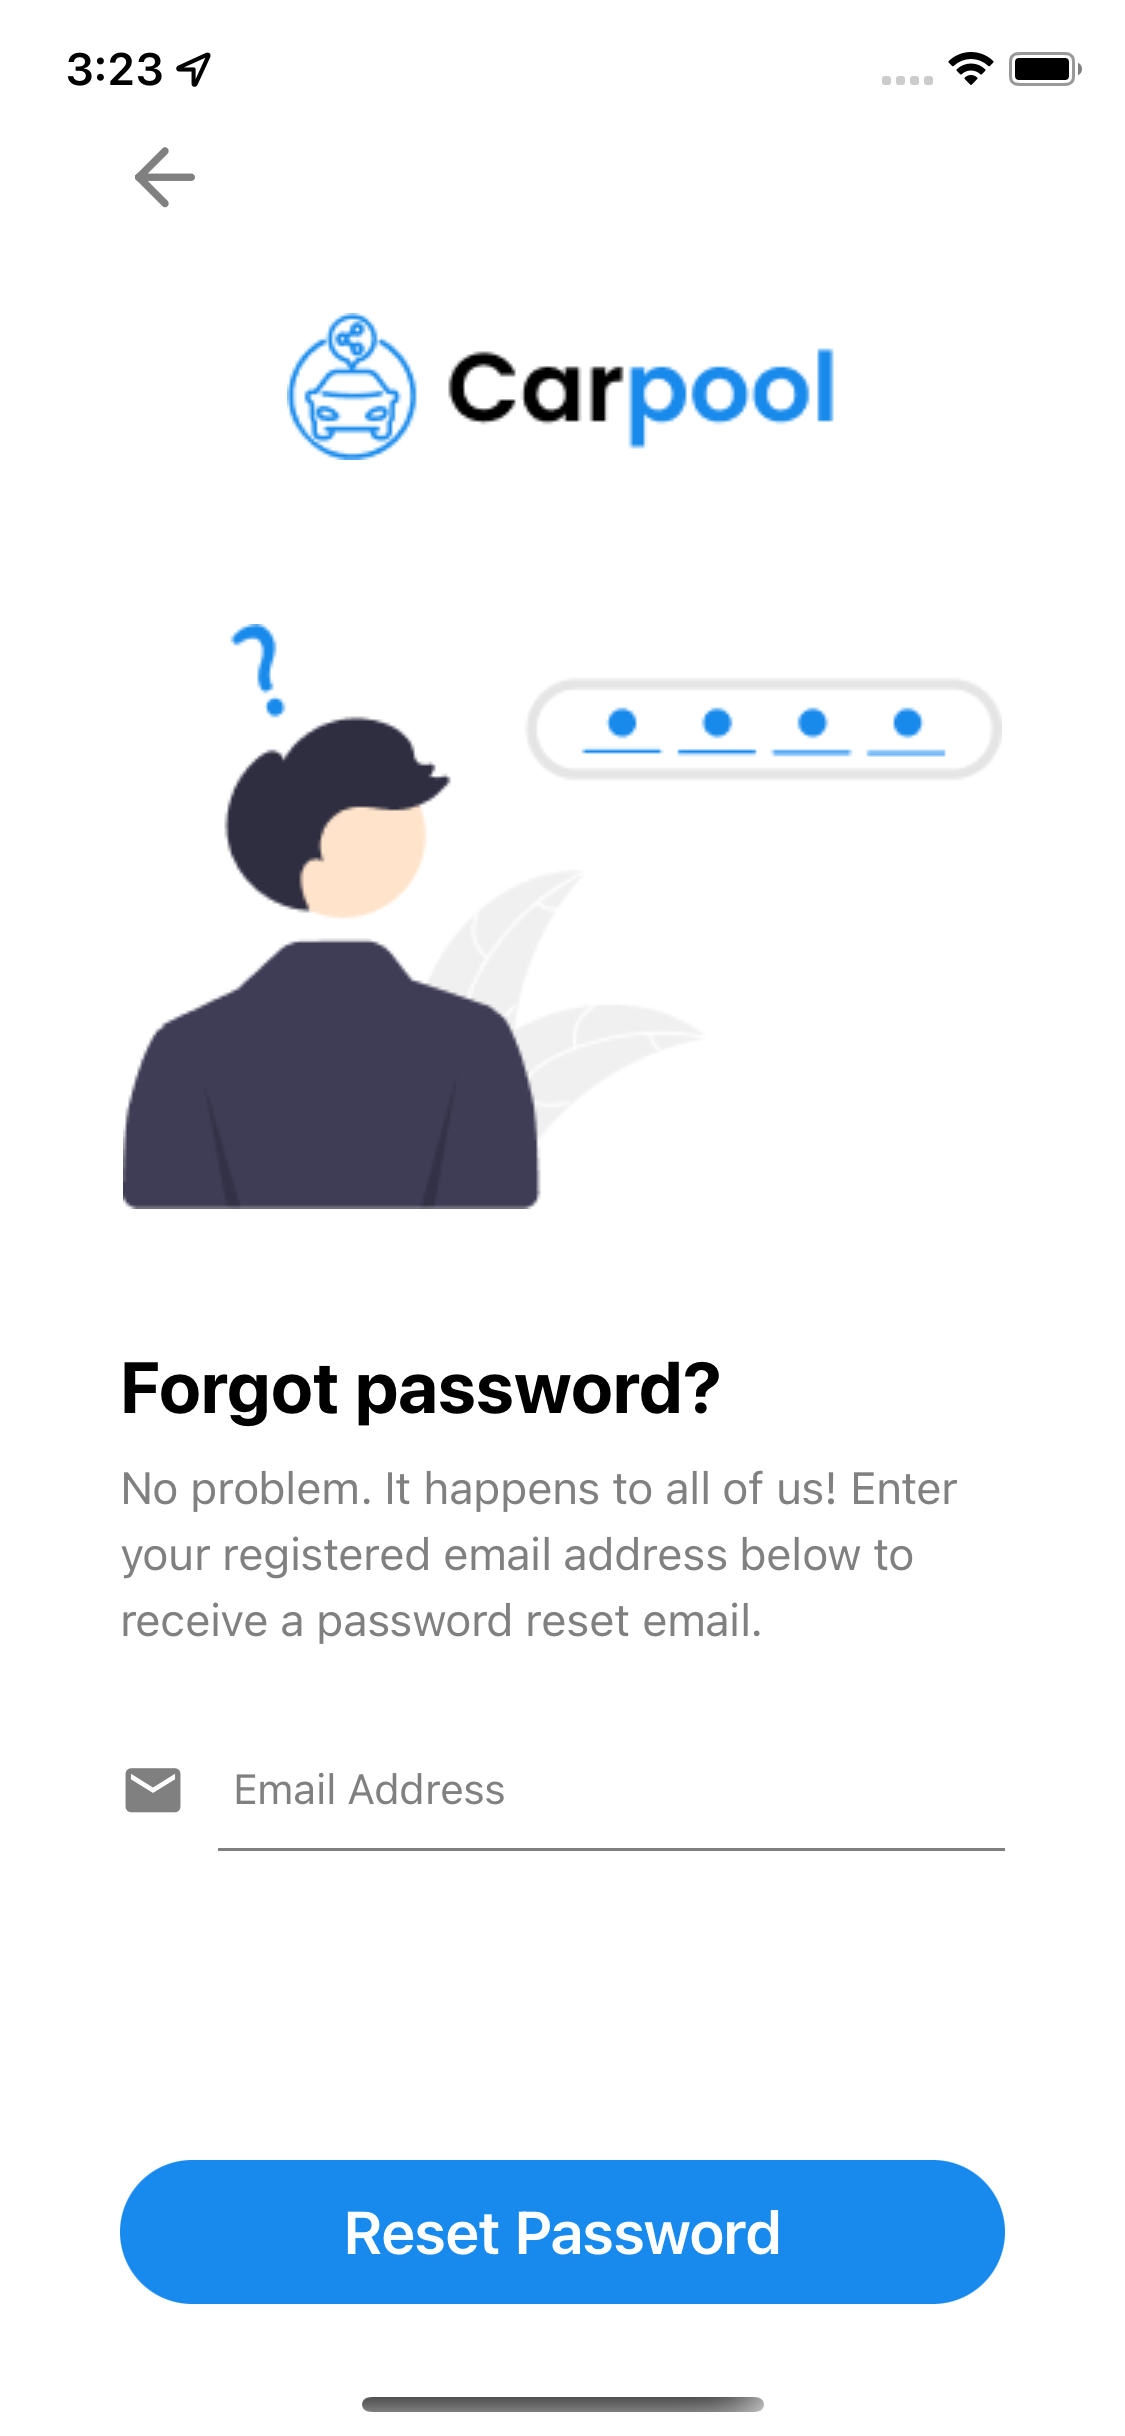
\includegraphics[height=10cm]{images/Simulator Screen Shot - iPhone X - 2022-06-10 at 03.23.17.png}
\end{center}
\vspace{1cm}

\subsection{Trips}
\subsubsection{Book Trip}
\begin{center}
  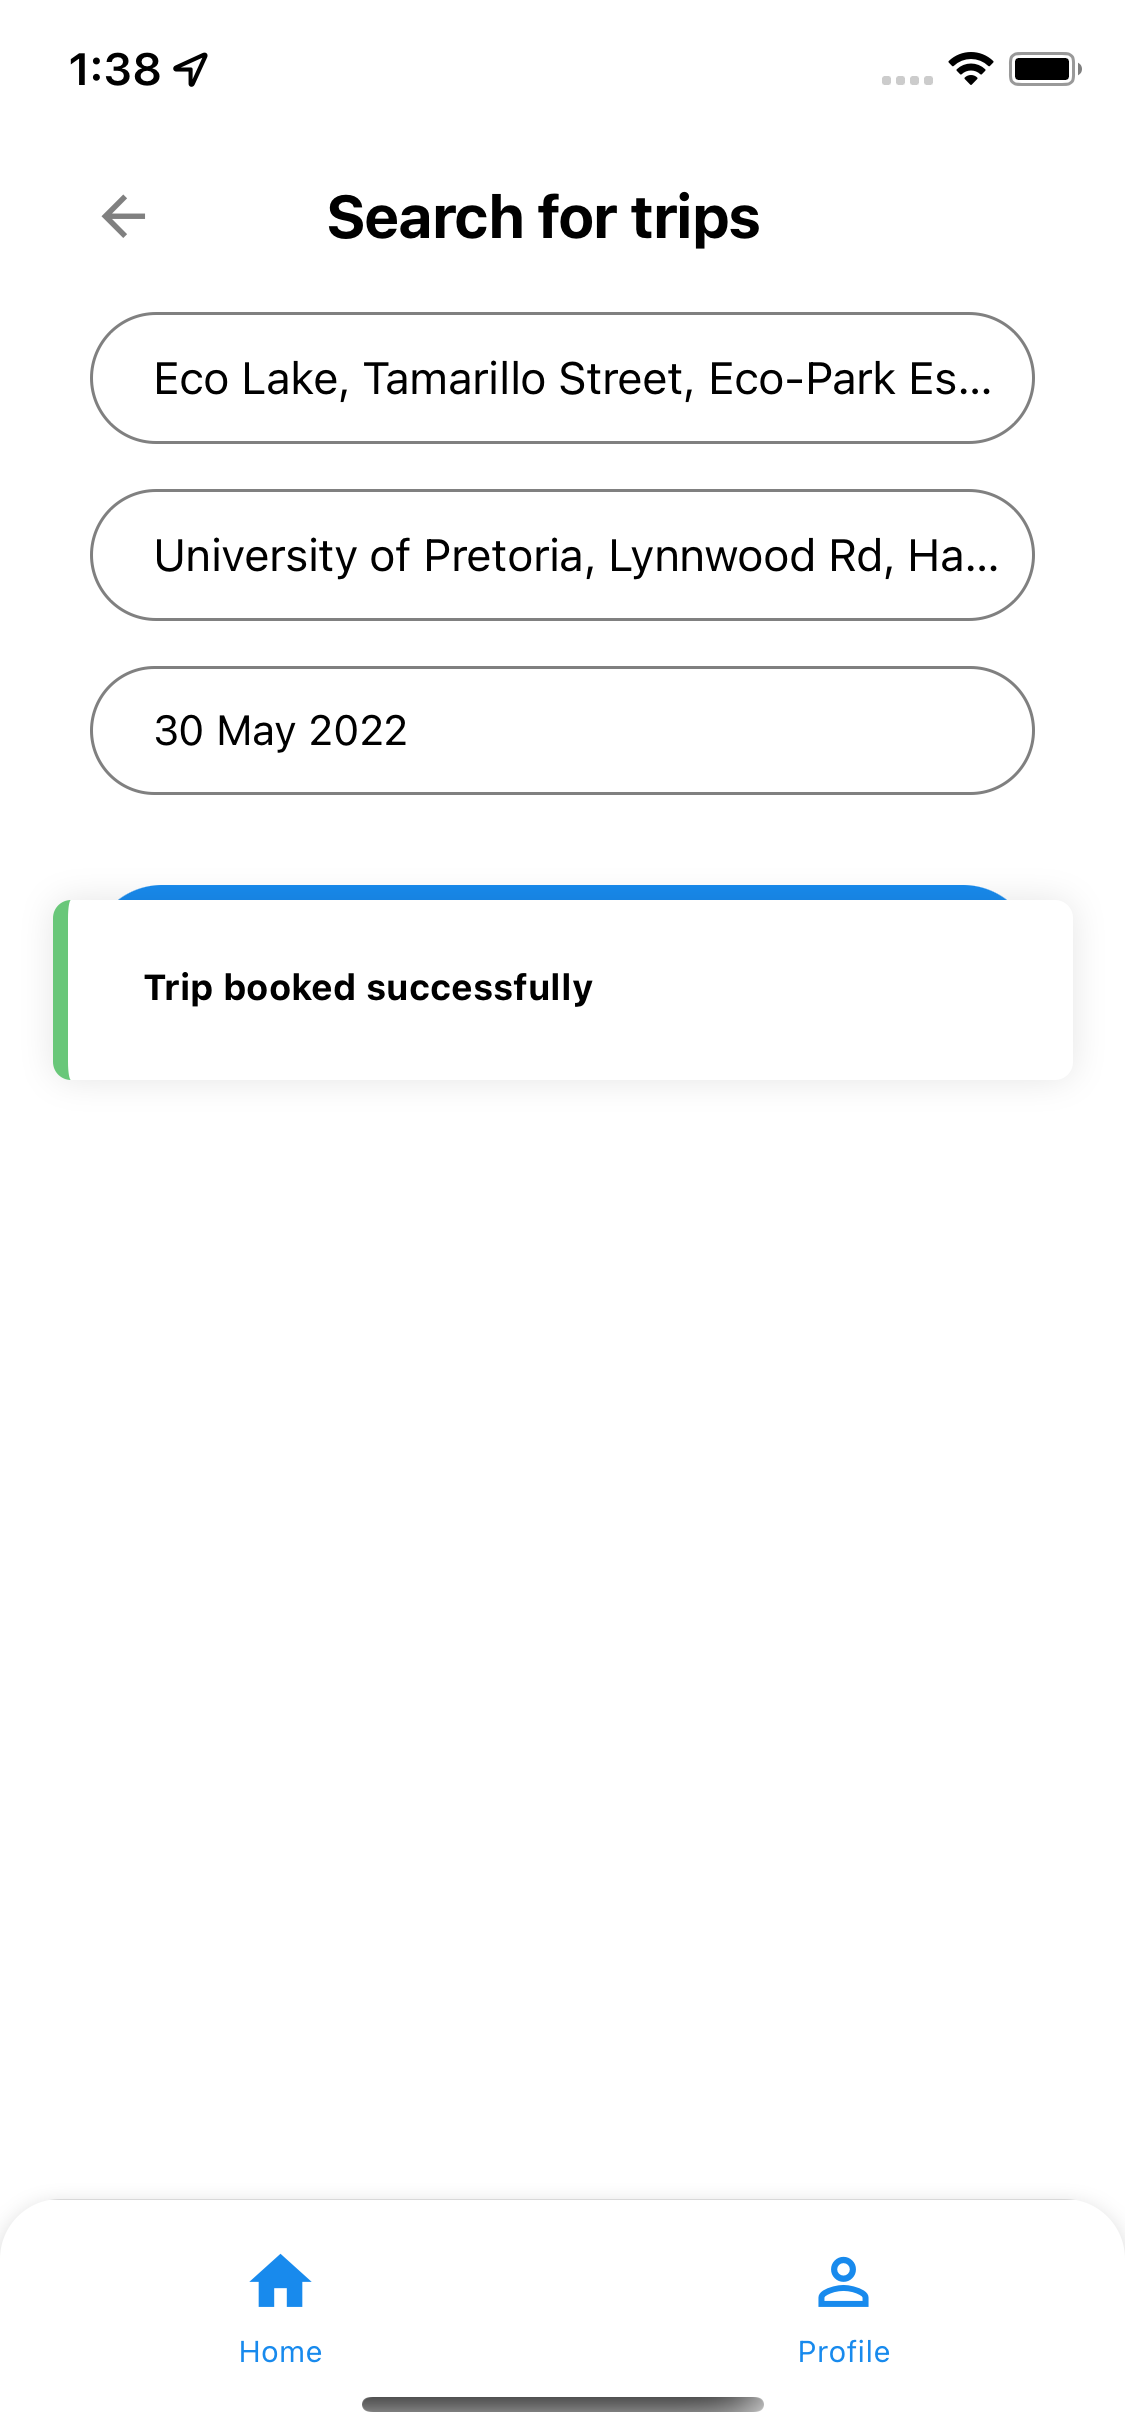
\includegraphics[height=10cm]{images/book_trip.png}
\end{center}
\subsubsection{Create Trip}
\begin{center}
  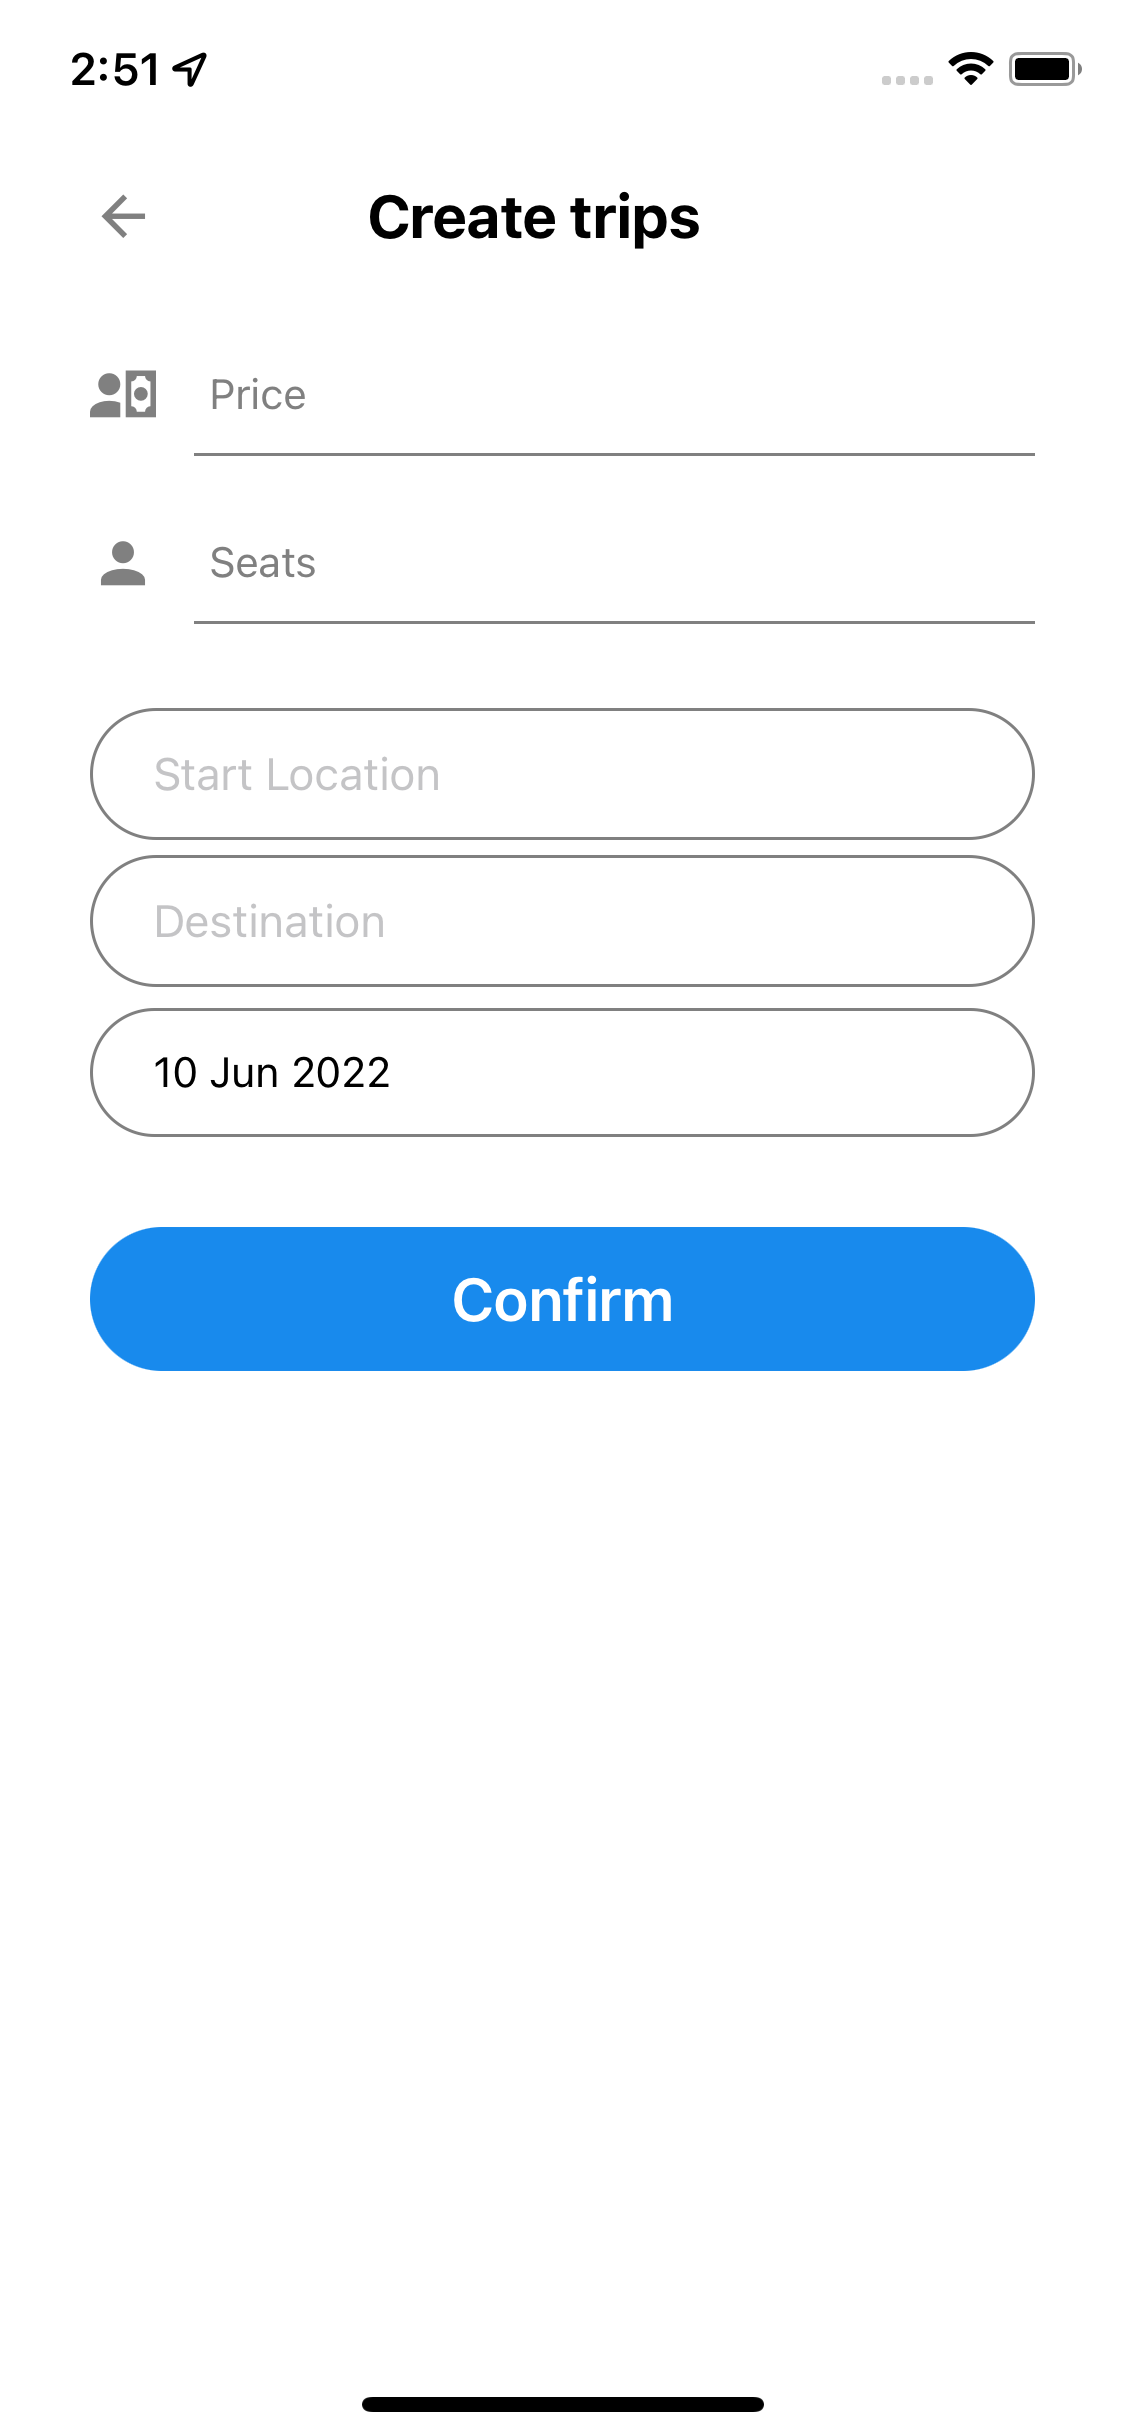
\includegraphics[height=10cm]{images/create_trip.png}
\end{center}
\vspace{1cm}
\subsubsection{Search Trip}
\begin{center}
  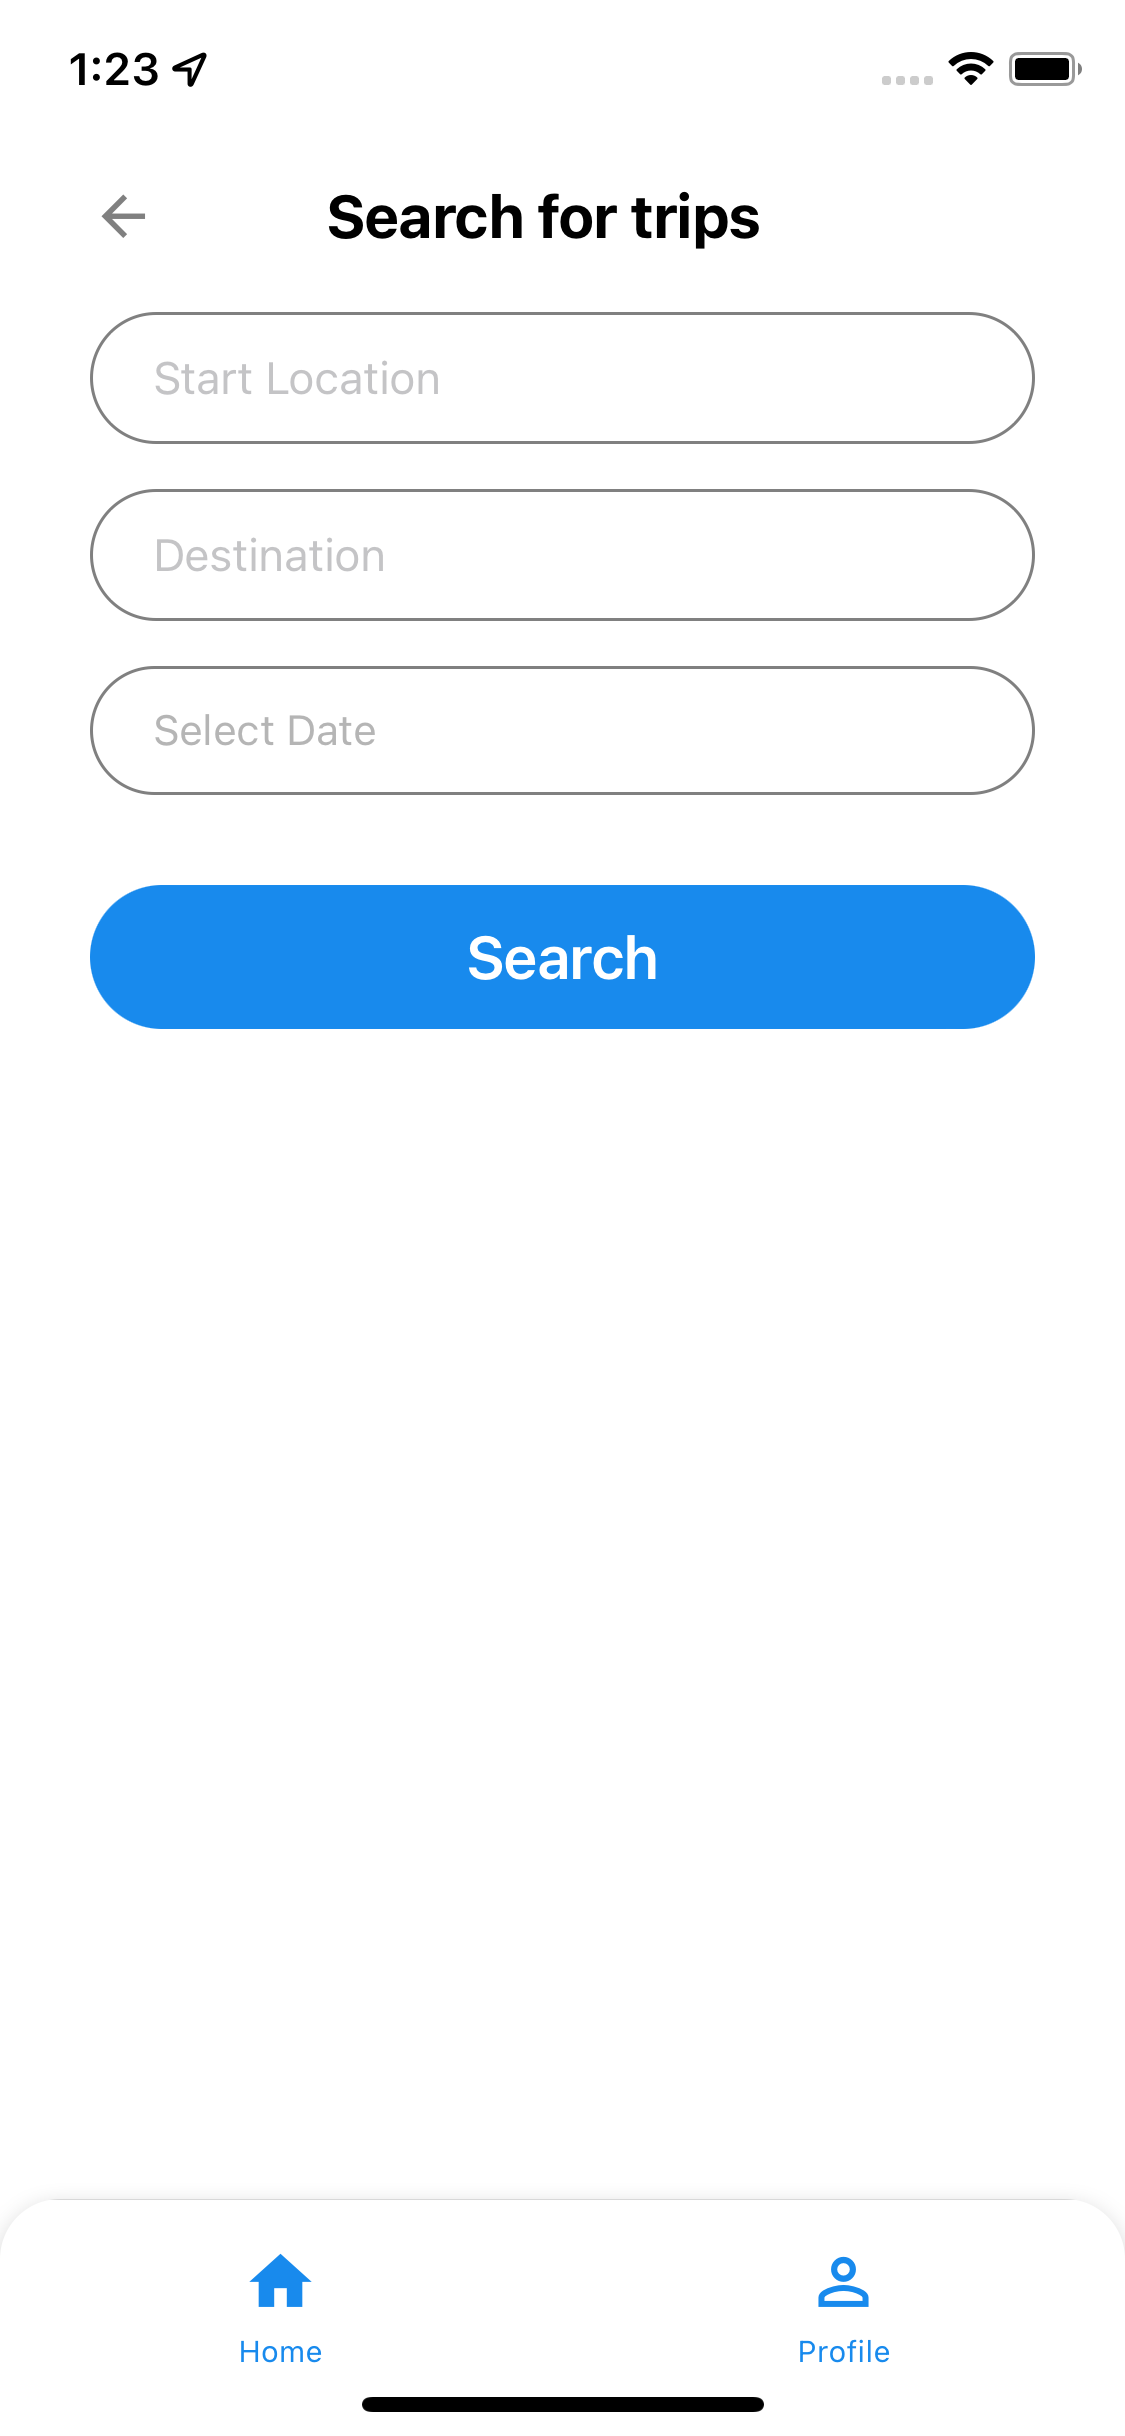
\includegraphics[height=10cm]{images/search_trips.png}
\end{center}
\vspace{1cm}

\subsection{Profiles}
\subsubsection{Edit Profile}
\begin{center}
  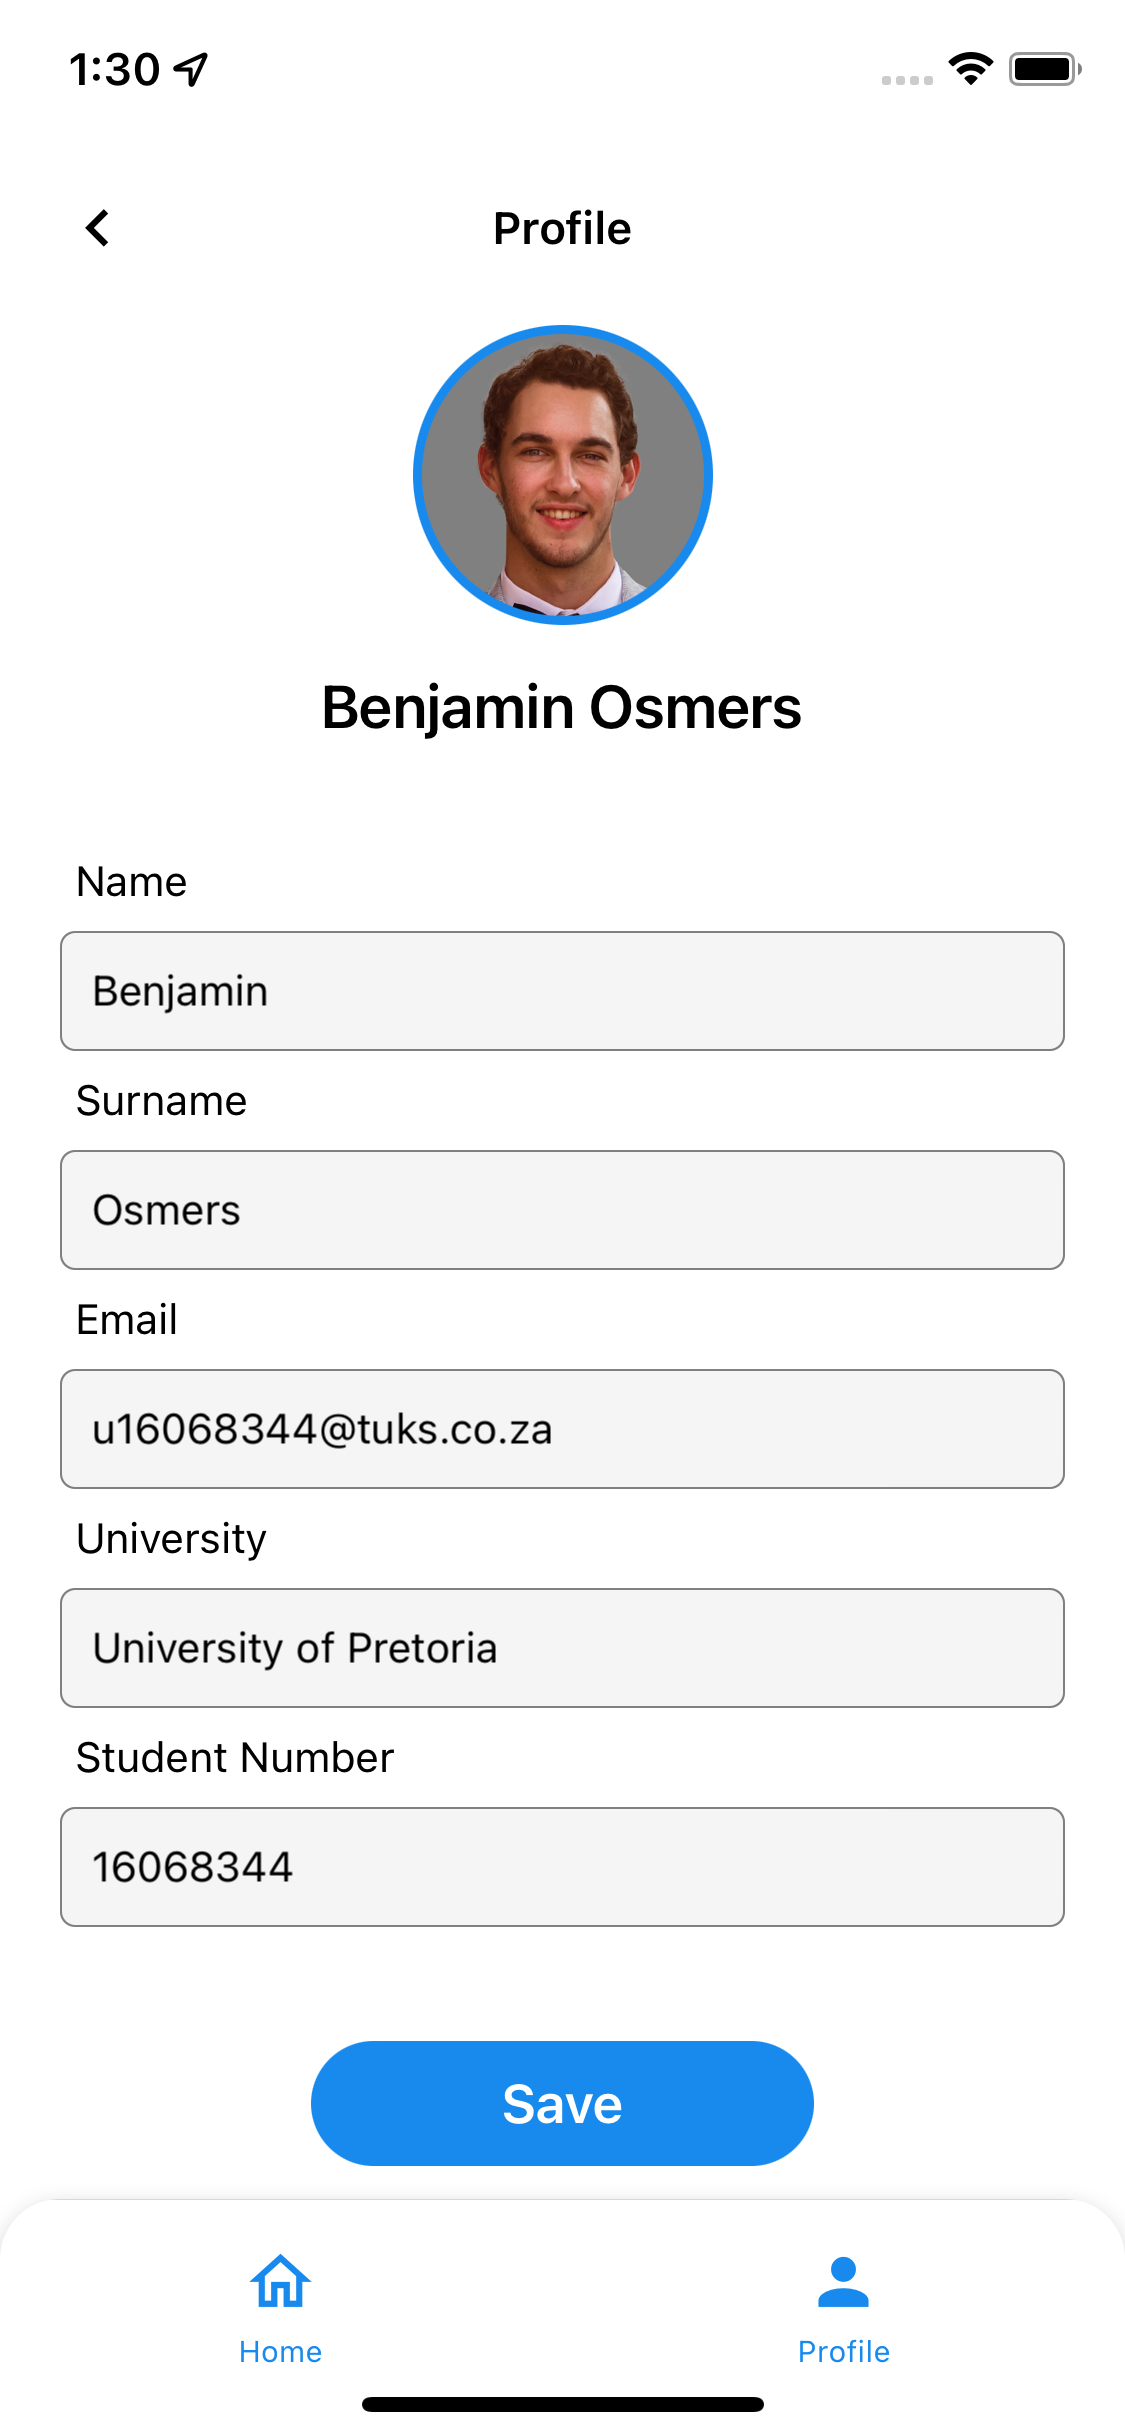
\includegraphics[height=10cm]{images/edit_profile.png}
\end{center}
\subsubsection{View Other profiles}
\begin{center}
  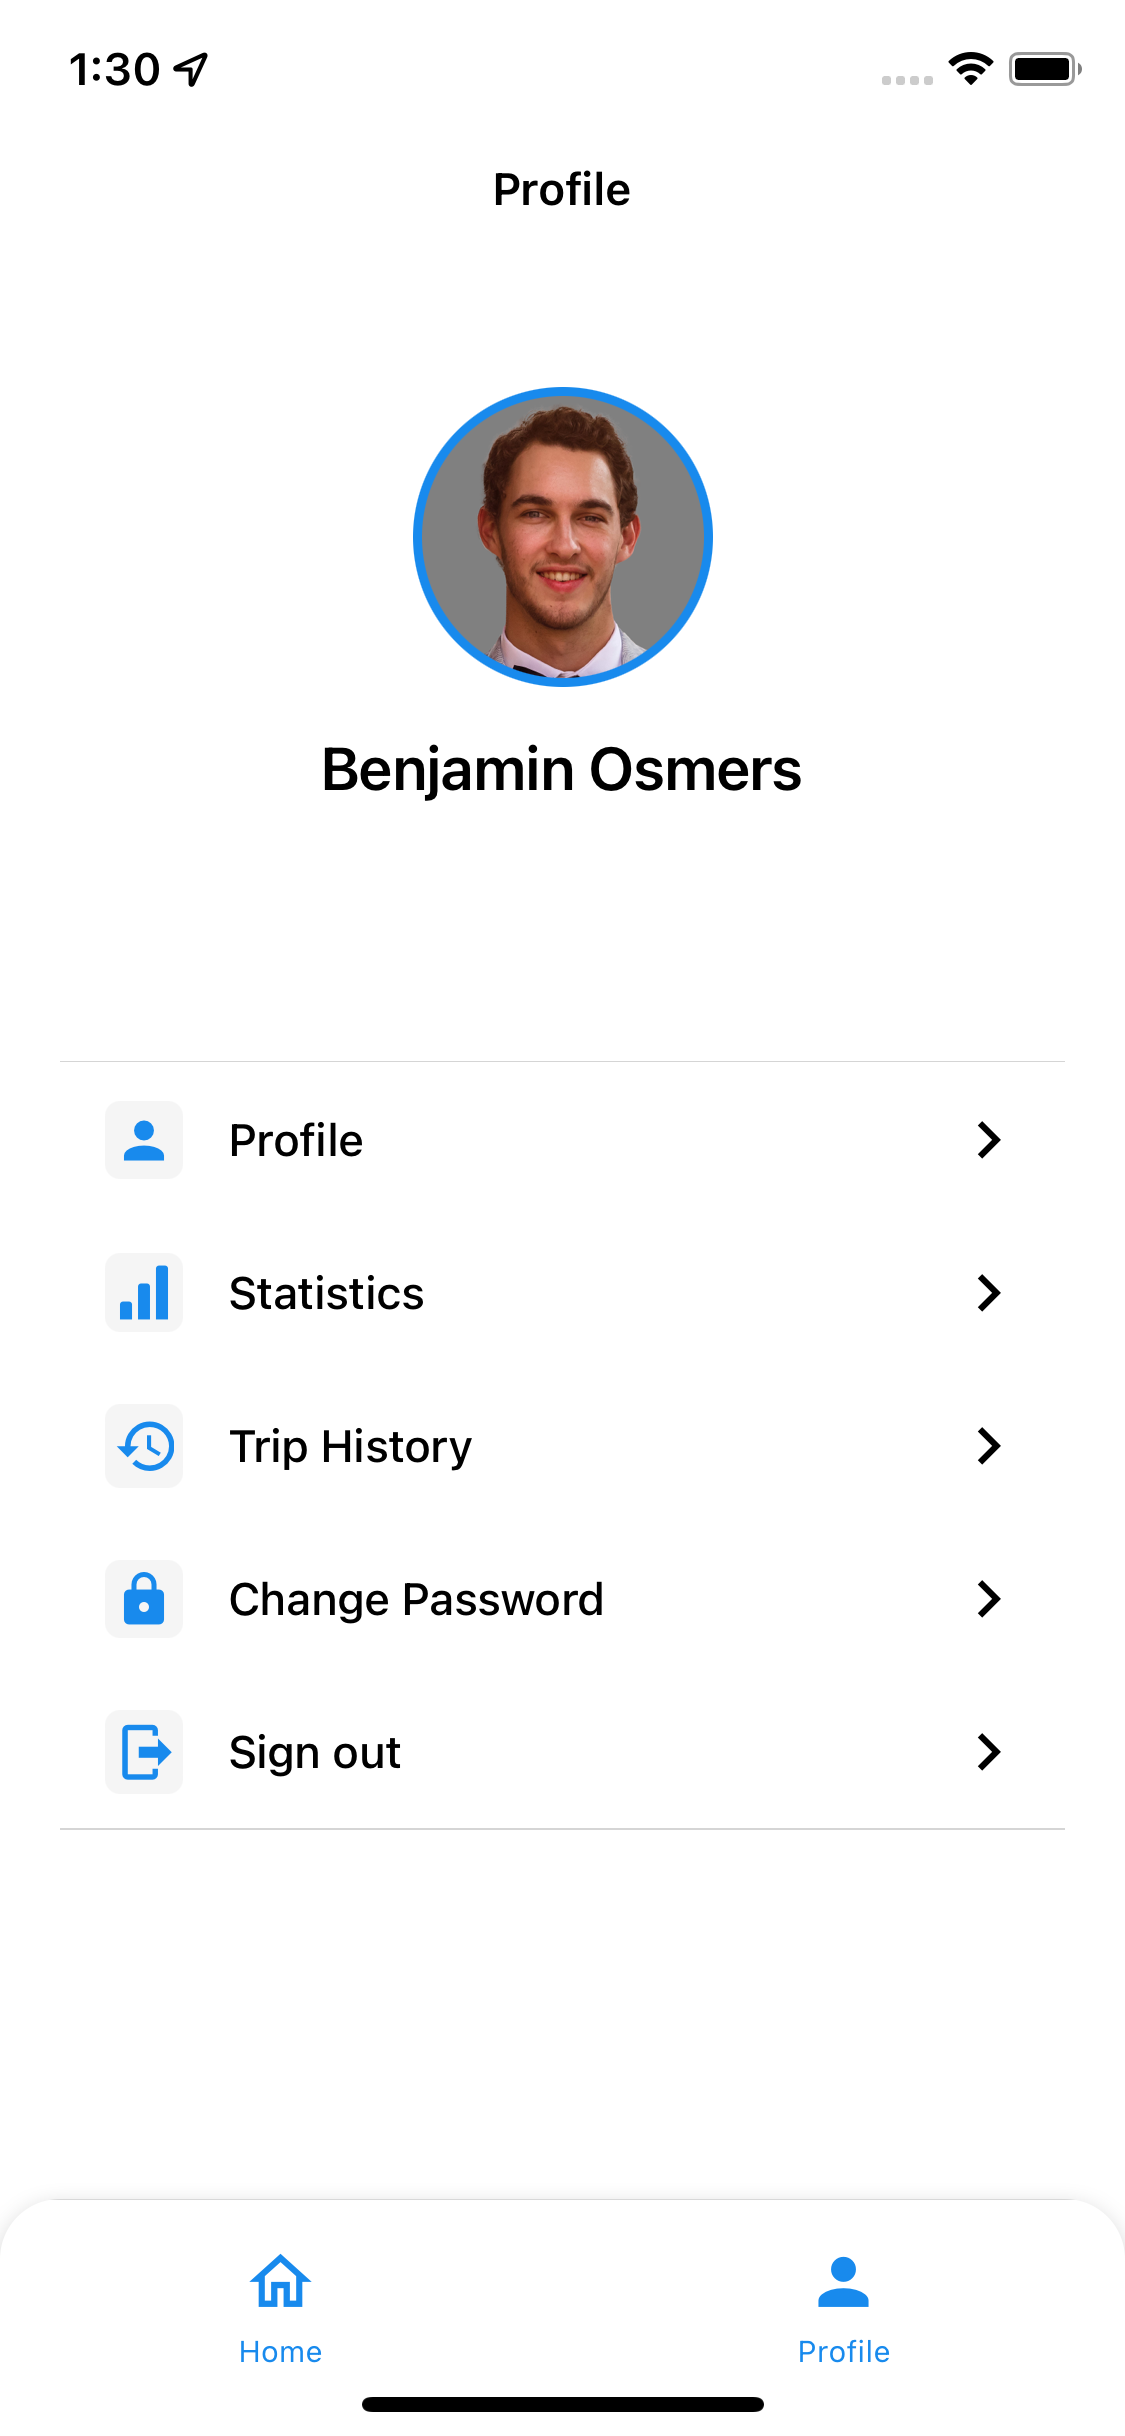
\includegraphics[height=10cm]{images/view_profile.png}
\end{center}
\vspace{1cm}

\subsection{History}
\subsubsection{Passenger History}
\begin{center}
  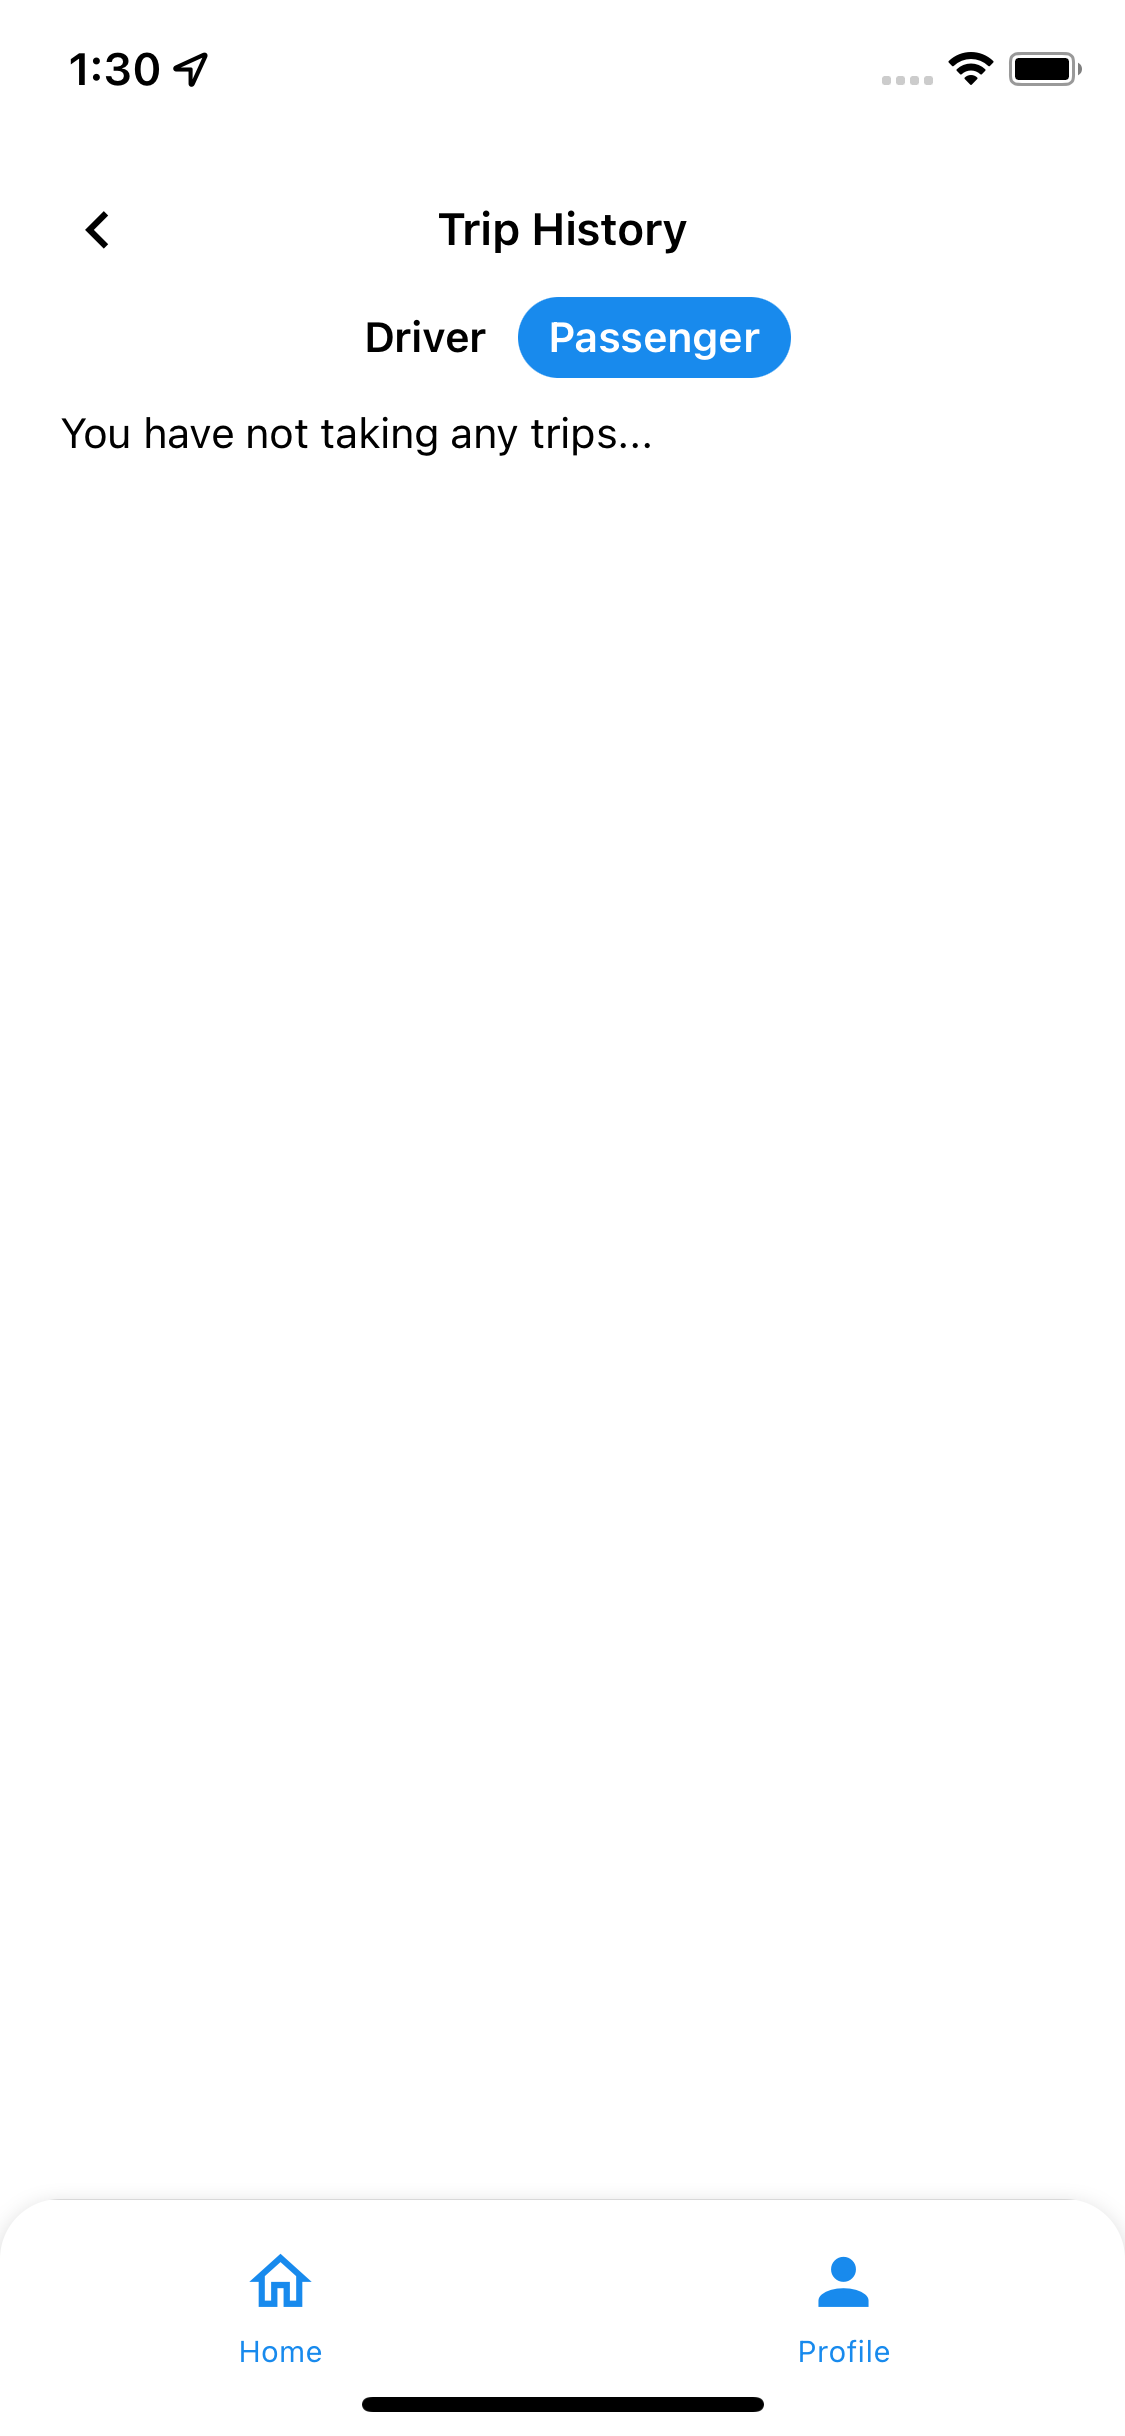
\includegraphics[height=10cm]{images/history_passenger.png}
\end{center}
\subsubsection{Driver History}
\begin{center}
  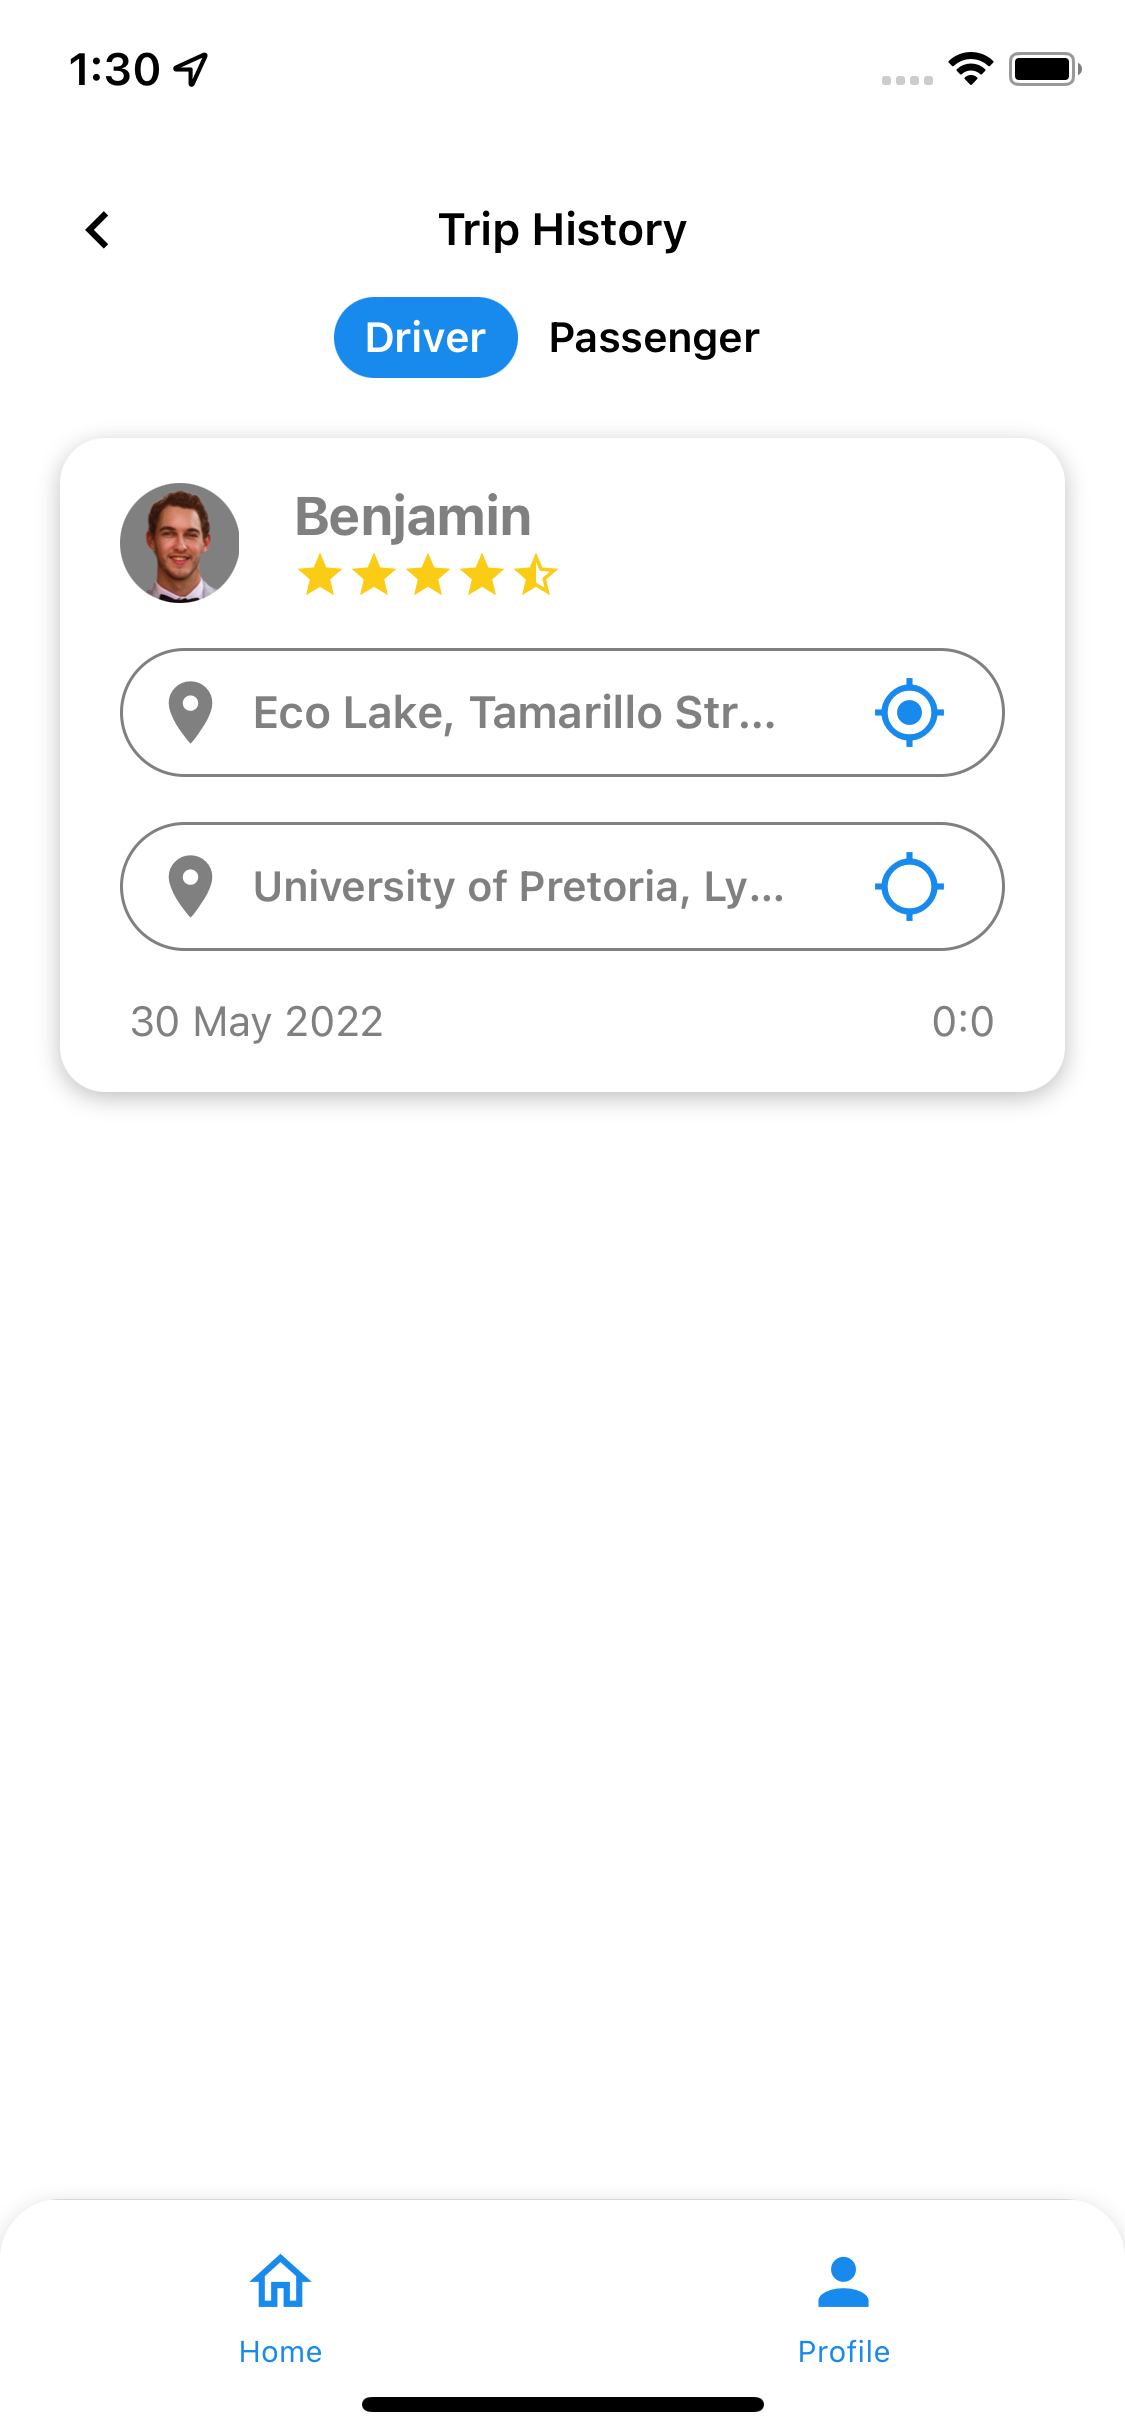
\includegraphics[height=10cm]{images/history_driver.png}
\end{center}
\vspace{1cm}

\subsection{Maps}
\subsubsection{Map direction}
\begin{center}
  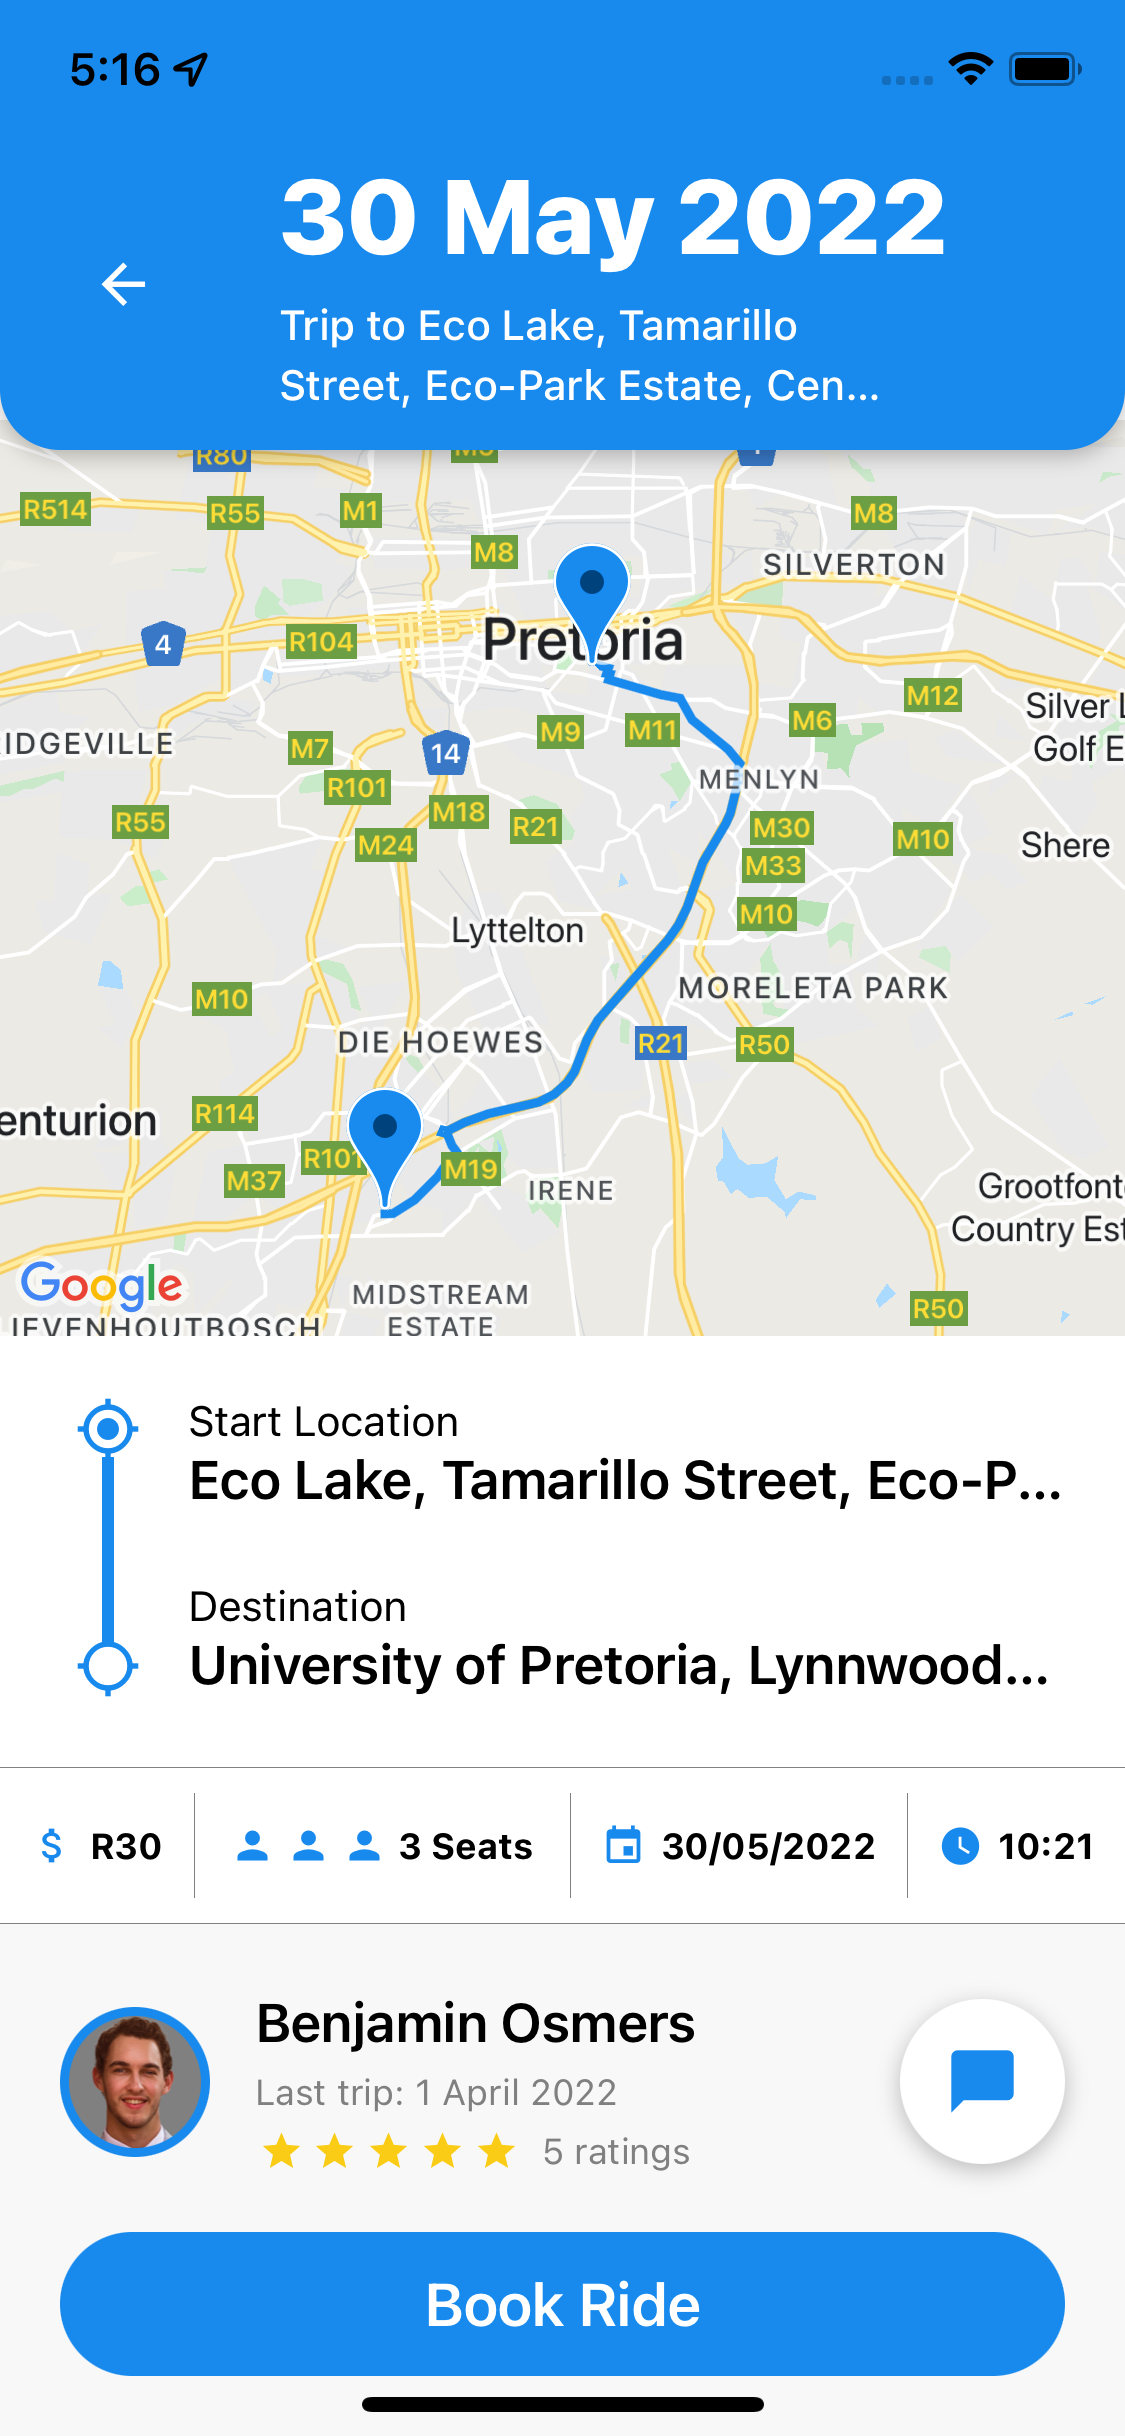
\includegraphics[height=10cm]{images/map_directions.png}
\end{center}
\subsubsection{Map display}
\begin{center}
  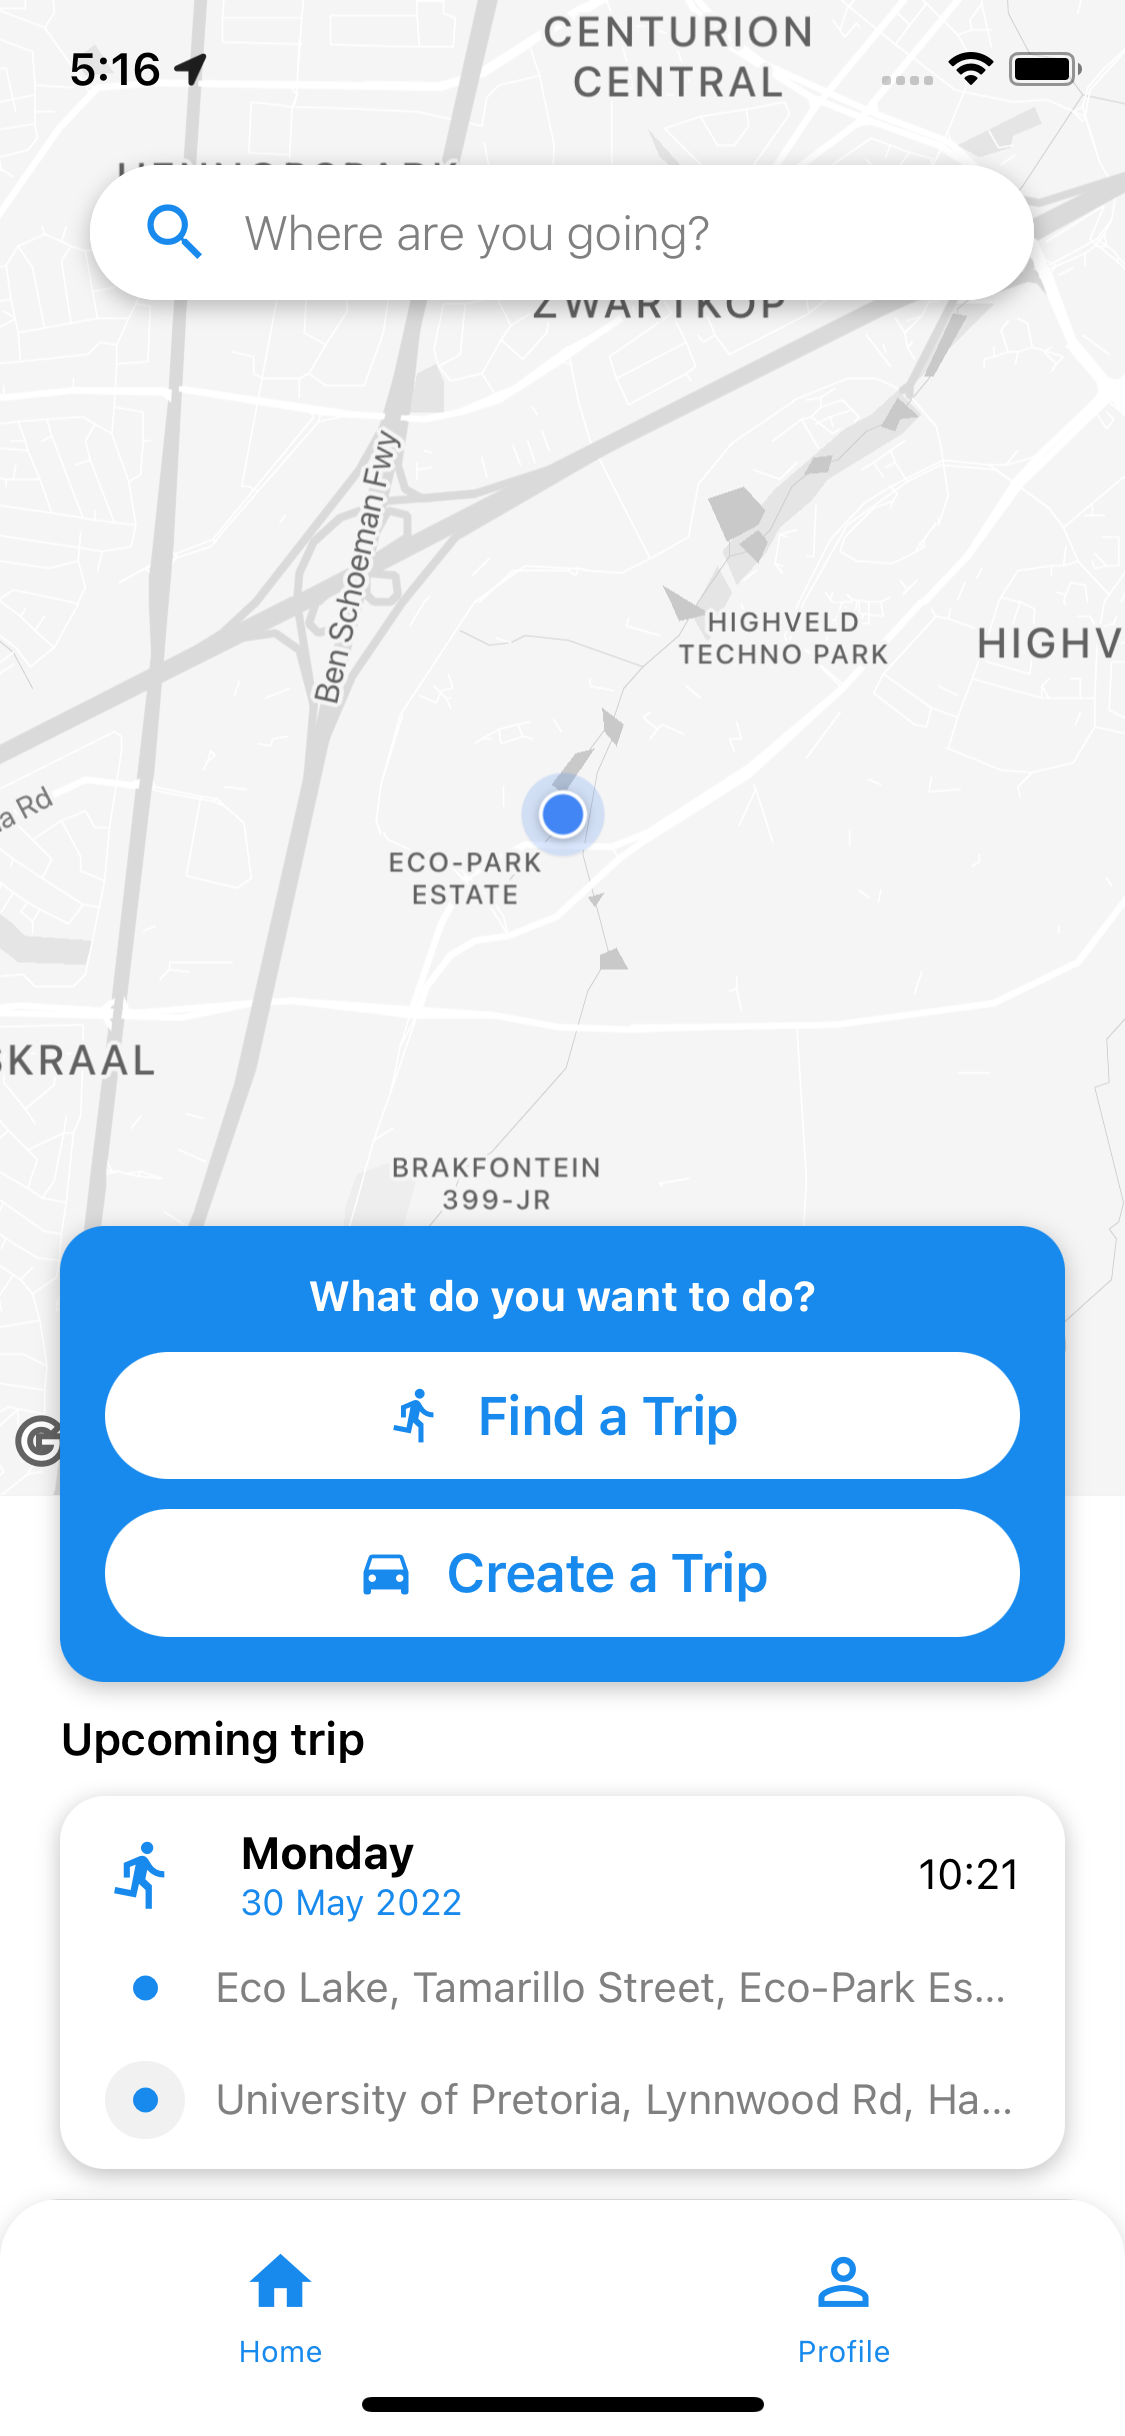
\includegraphics[height=10cm]{images/map_display.png}
\end{center}
\vspace{1cm}

\end{document}